\section{Physical Analysis}
\label{sec:physics}

\subsection{Derived Parameters}
\label{sec:derived-params}

From the mean fitted value $a = 765.35$ and the known hardware constants
($\SH = \SI{130}{\volt/\tesla}$, $\kA = \SI{0.3614}{\ampere/\volt}$,
$\Nc = 50$), we recover the magnetic circuit parameters using
\cref{eq:kpole,eq:Ra}:
\begin{align}
\kpole &= \frac{4\pi \times 765.35^2}{130 \times 0.3614 \times 10^{12}}
        = 1.57 \times 10^{-7} \;\text{Wb/A}, \\
\Ra    &= \frac{50}{1.57 \times 10^{-7}}
        = 3.19 \times 10^{8} \;\text{A/Wb}.
\end{align}

\Cref{tab:physical-params} compares these results with the quadrupole
actuator of Zhang and Menq~\cite{Zhang2010} and the hexapole actuator of
Menq~\cite{Menq2011}.

% Table 3: Physical parameters — this work vs Menq
\begin{table}[htbp]
\centering
\caption{Comparison of magnetic actuator parameters. Note that $\Ra$ from
this work represents the total reluctance $R_\mathrm{total}$ (pole + gap +
air return) of a single yokeless pole, whereas Menq's $\Ra$ is the
air-gap reluctance only (with a ferromagnetic yoke providing a low-reluctance
return path). Direct comparison of $\Ra$ is therefore not meaningful;
the offset $b$ is the appropriate figure of merit.}
\label{tab:physical-params}
\begin{tabular}{@{}lccc@{}}
\toprule
Parameter & This work & Menq 2010 \cite{Zhang2010} & Menq 2011 \cite{Menq2011} \\
\midrule
Configuration & Hexapole (no yoke) & Quadrupole (yoke) & Hexapole (yoke) \\
$\Nc$ (turns)           & 50     & 200    & 200 \\
$\rtip$ (\si{\um})      & 5      & 40     & 40 \\
$\kpole$ (Wb/A)         & $1.57 \times 10^{-7}$ & --- & --- \\
$\Ra$ (A/Wb)            & $3.19 \times 10^{8}$\textsuperscript{a} & $1.8 \times 10^{9}$\textsuperscript{b} & $2.8 \times 10^{9}$\textsuperscript{b} \\
$b$ or $l$ (\si{\um})   & 1979   & 405    & --- \\
$K_I$                   & 1      & ---    & --- \\
\bottomrule
\multicolumn{4}{@{}l}{\footnotesize \textsuperscript{a} $R_\mathrm{total}$ (no yoke). \textsuperscript{b} $R_\mathrm{air\text{-}gap}$ (with yoke).}
\end{tabular}
\end{table}


\textbf{Important caveat regarding $\Ra$:} The value $\Ra = 3.19 \times 10^8$
A/Wb from this work represents the \emph{total} reluctance
$R_\mathrm{total} = R_\mathrm{pole} + R_\mathrm{gap} + R_\mathrm{return\;air}$
of the magnetic circuit for a single yokeless pole, where the flux must return
through the surrounding air. In contrast, Menq's values
($1.8 \times 10^9$ for the quadrupole, $2.8 \times 10^9$ for the hexapole)
represent the \emph{air-gap reluctance only}, because the ferromagnetic yoke
provides a low-reluctance return path. These two quantities are fundamentally
different and cannot be directly compared.

The offset parameter $b$ is therefore the more meaningful figure of merit:
it directly quantifies how effectively the magnetic circuit concentrates flux
at the pole tip, regardless of the circuit topology.

\subsection{Field, Gradient, and Force Profiles}
\label{sec:force-profiles}

Using the derived $\kpole$ and a peak current of
$I = \kA \times \Vda = 0.3614 \times 2.0 = \SI{0.723}{\ampere}$,
we compute the magnetic field $B(x)$, field gradient $|\mathrm{d}B/\mathrm{d}x|$,
and magnetic force $\Fmag(x)$ on a paramagnetic bead.

The force is computed for a Dynabeads M-450 bead
($d = \SI{4.5}{\um}$, $\chi_\mathrm{vol} = 0.4$,
$\chitot = 3\chi/(3+\chi) = 0.353$ accounting for sphere demagnetization)
using \cref{eq:force}.

\Cref{fig:physics} shows the 2$\times$2 analysis: $B(x)$,
$|\mathrm{d}B/\mathrm{d}x|$, $\Fmag(x)$, and the force-to-thermal-noise
ratio $\Fmag / \Fthermal$.

\begin{figure}[htbp]
\centering
\includegraphics[width=0.85\textwidth]{../results/Charge_NTU/figures/Charge_Physics_Analysis.png}
\caption{Physical analysis. Top-left: magnetic field $B(x)$.
Top-right: field gradient. Bottom-left: force on a
$\SI{4.5}{\um}$ bead. Bottom-right: force SNR
($\Fmag / \Fthermal$); the dashed line marks unity.}
\label{fig:physics}
\end{figure}

% Table 4: Force estimates at representative distances
% Bead: Dynabeads M-450, d = 4.5 um, chi_vol = 0.4
% I_peak = k_A * V_DA = 0.3614 * 2.0 = 0.7228 A
\begin{table}[htbp]
\centering
\caption{Magnetic field and force estimates at representative distances.
Current $I = \SI{0.723}{\ampere}$ ($\Vda = \SI{2.0}{\volt}$, $\kA = \SI{0.3614}{\ampere/\volt}$).
Bead: Dynabeads M-450 ($d = \SI{4.5}{\um}$, $\chi_\mathrm{vol} = 0.4$).
$\Fthermal = \SI{0.0037}{\pico\newton}$ ($T = \SI{300}{\kelvin}$, $\Delta t = \SI{1}{\second}$).}
\label{tab:force-estimates}
\begin{tabular}{@{}rcccc@{}}
\toprule
$x$ (\si{\um}) & $B$ (mT) & $|\mathrm{d}B/\mathrm{d}x|$ (T/m) & $F$ (pN) & $F/\Fthermal$ \\
\midrule
10    & 2.296 & 2.310 & 0.0210 & 5.67 \\
100   & 2.118 & 1.020 & 0.0086 & 2.31 \\
500   & 1.490 & 0.367 & 0.0022 & 0.59 \\
1000  & 0.967 & 0.130 & 0.0005 & 0.14 \\
2000  & 0.456 & 0.023 & 0.0000 & 0.01 \\
\bottomrule
\end{tabular}
\end{table}


Key observations from \cref{tab:force-estimates}:
\begin{itemize}
\item At the closest measured distance ($x = \SI{10}{\um}$),
$B = \SI{2.3}{\milli\tesla}$, well within the EQ-730L linear range of
$\pm\SI{15}{\milli\tesla}$.
\item The force is sub-piconewton everywhere:
$\Fmag(\SI{10}{\um}) = \SI{0.021}{\pico\newton}$.
\item The force exceeds the thermal noise floor
($\Fthermal = \SI{0.0037}{\pico\newton}$) only for
$x \lesssim \SI{609}{\um}$.
\end{itemize}

\subsection{Comparison with Yoke Design}
\label{sec:yoke-comparison}

The fundamental difference between the yokeless actuator studied here and
the yoke-based designs of Menq is captured by the offset parameter:
$b_\mathrm{NTU} = \SI{1979}{\um}$ versus
$b_\mathrm{Menq} = l = \SI{405}{\um}$.

\Cref{fig:yoke-comparison} overlays the normalized field decay
$H(x)/H(0) = b^2/(x+b)^2$ for both designs. The yoke design maintains a
stronger field at all distances because its smaller $b$ concentrates the
flux closer to the tip.

\begin{figure}[htbp]
\centering
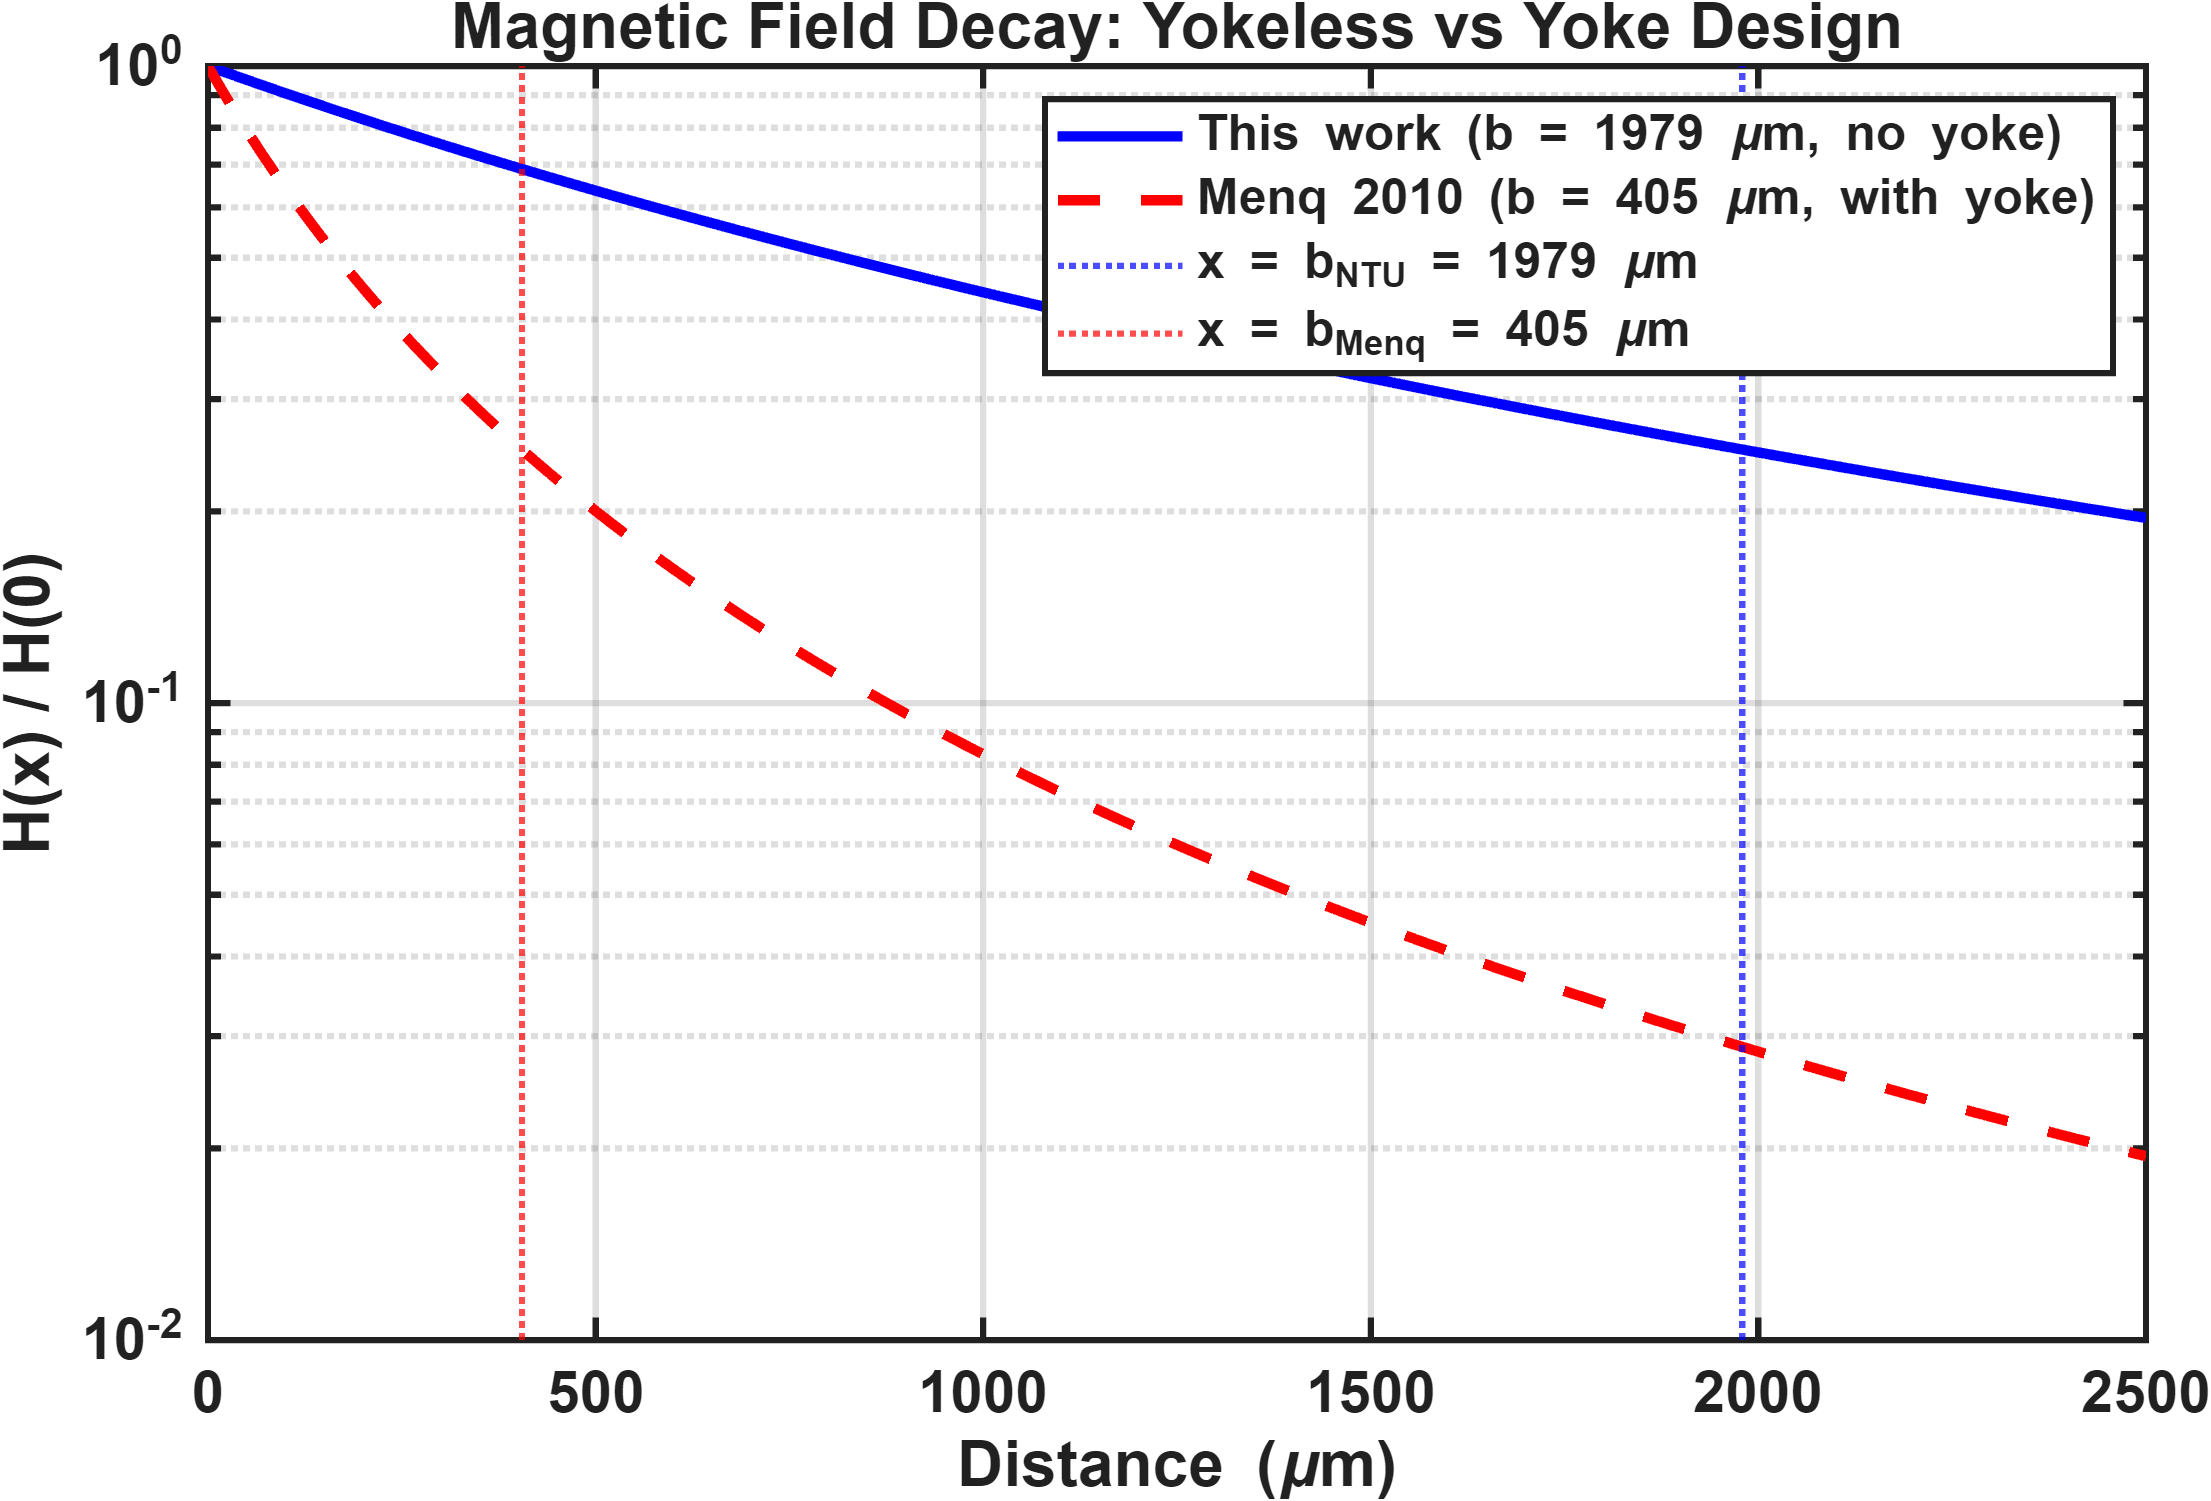
\includegraphics[width=0.7\textwidth]{figures/yoke_comparison.png}
\caption{Normalized field decay for the yokeless actuator
($b = \SI{1979}{\um}$, this work) and the yoke-based quadrupole
($b = \SI{405}{\um}$, Menq~\cite{Zhang2010}).}
\label{fig:yoke-comparison}
\end{figure}

Since the force scales as $F \propto B \cdot |\mathrm{d}B/\mathrm{d}x|
\propto 1/(x+b)^5$, the force suppression at the pole tip
($x = \rtip = \SI{5}{\um}$) is
\begin{equation}
\frac{F_\mathrm{real}}{F_\mathrm{ideal}} = \left(\frac{\rtip}{\rtip + b}\right)^5
\approx \left(\frac{5}{1984}\right)^5 \approx 10^{-14},
\end{equation}
where $F_\mathrm{ideal}$ is the force from a true point charge at the tip
surface. This enormous suppression factor explains why the yokeless
configuration produces sub-piconewton forces: the flux is spread over a
volume far larger than the tip geometry.
